\section{Discussion}

The hollow interior of the triangles considered in this work is needed for two reasons: (1) $W\ll L$ is required for bulk-edge correspondence based on 1D topology to hold; (2) A finite $W$ is needed to gap out the chiral edge states of a 2D spinless $p$-wave superconductor based on which Eq.~\eqref{eq:Hribbon} is written. The latter is not essential if one does not start with a spinless $p$-wave supercondutor but a more realistic model such as the Rashba+Zeeman+$s$-wave pairing model. On the other hand, the former constraint may also be removed if one uses the Kitaev triangle. Nonetheless, an effective 3-site Kitaev triangle may emerge as the effective theory of triangular structures if a three-orbital low-energy Wannier basis can be isolated, similar to the continuum theory of moir\'{e} structures. We also note in passing that the corner MZM in our triangles appear due to different reasons from that in higher-order topological superconductors \cite{wangEvidenceMajoranaBound2018,pahomiBraidingMajoranaCorner2020}.

\begin{figure}[!hb]
  \begin{tikzpicture}
    \node[inner sep=0pt] (figure) at (0,0)
    {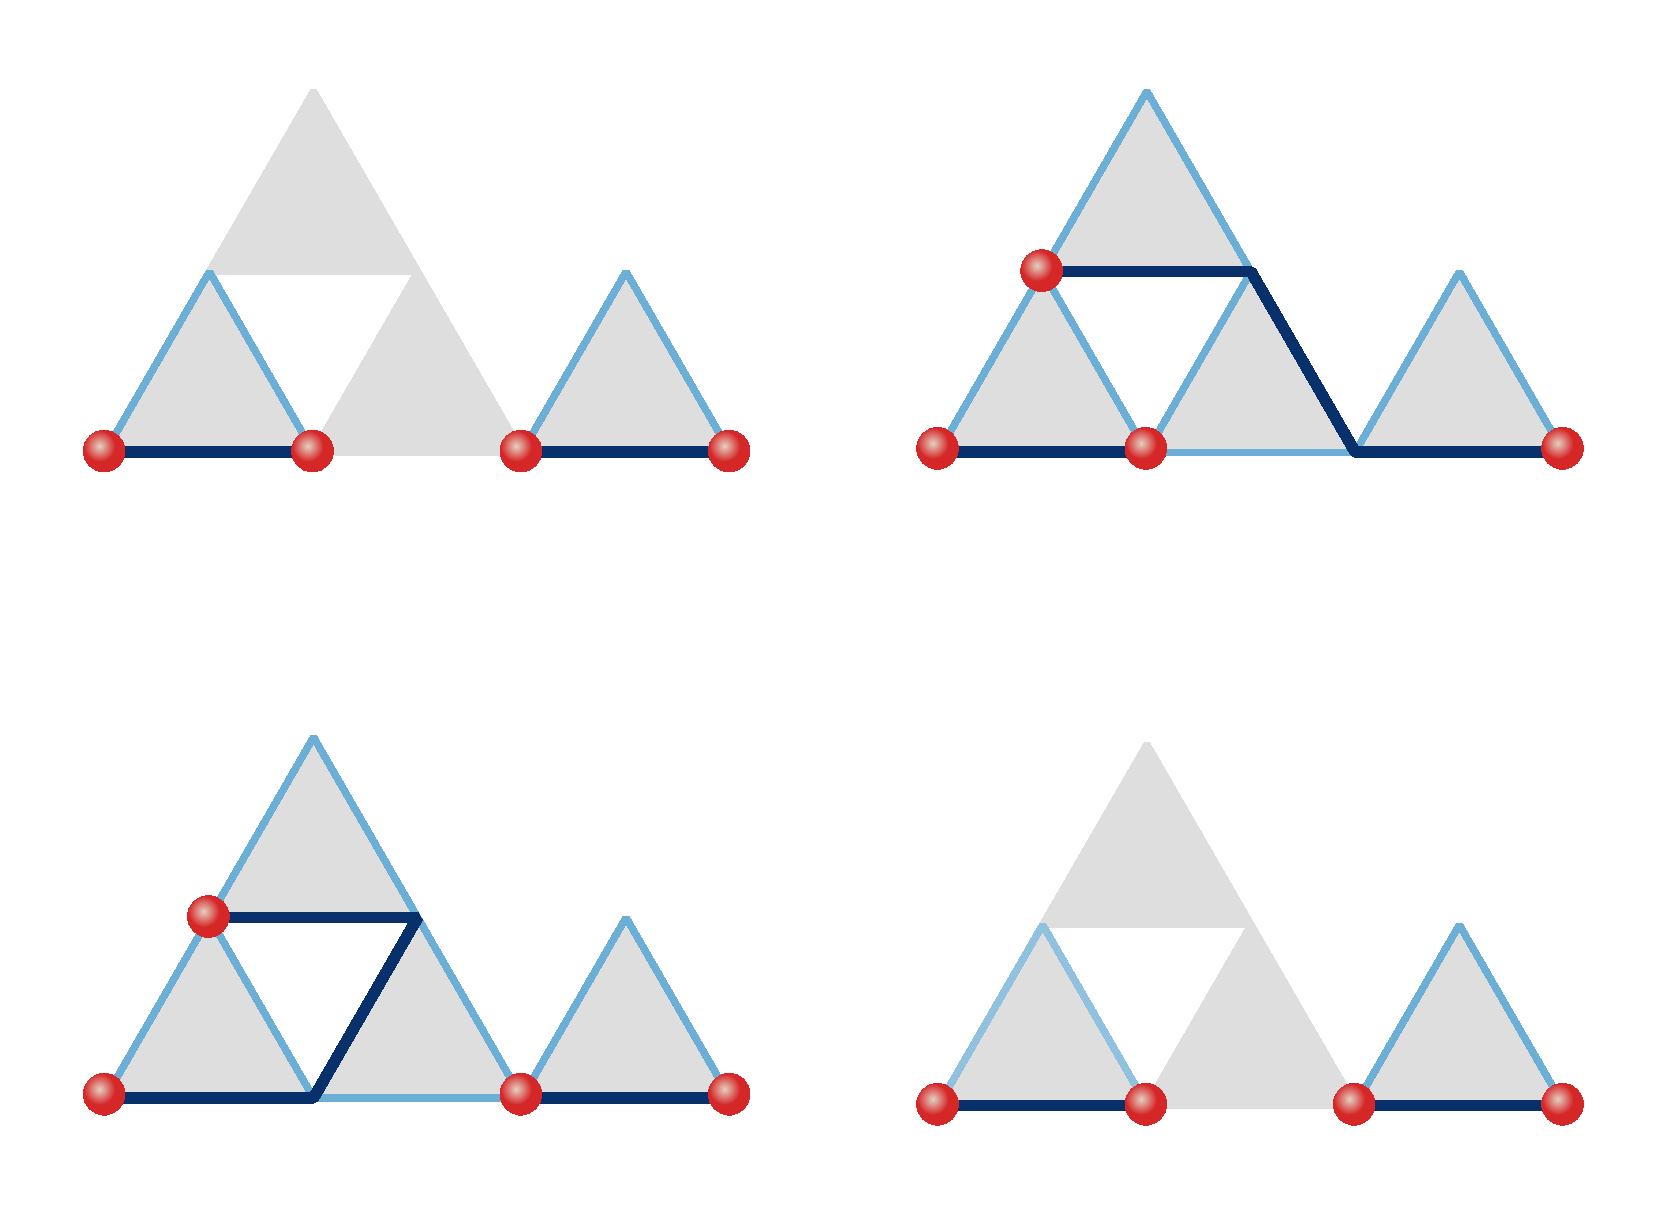
\includegraphics[width=0.90\textwidth]{./figures/4-mf-swap-2-3.pdf}};

    \node[inner sep=0pt] (a) at (-8,5.50) {(a)};
    \node[inner sep=0pt] (b) at (0.2,5.50) {(b)};
    \node[inner sep=0pt] (c) at (-8,-.50) {(c)};
    \node[inner sep=0pt] (d) at (0.2,-.50) {(d)};

    \node[inner sep=0pt] (gamma1) at (-6.6,0.95) {$\gamma_1$};
    \node[inner sep=0pt] (gamma2) at (-4.6,0.95) {$\gamma_2$};
    \node[inner sep=0pt] (gamma3) at (-2.8,0.95) {$\gamma_3$};
    \node[inner sep=0pt] (gamma4) at (-0.9,0.95) {$\gamma_4$};

    \node[inner sep=0pt] (gamma1) at (0.90,0.95) {$\gamma_1$};
    \node[inner sep=0pt] (gamma2) at (2.80,0.95) {$\gamma_2$};
    \node[inner sep=0pt] (gamma3) at (1.4,3.50) {$\gamma_3$};
    \node[inner sep=0pt] (gamma4) at (6.50,0.95) {$\gamma_4$};

    \node[inner sep=0pt] (gamma1) at (-6.6,-4.80) {$\gamma_1$};
    \node[inner sep=0pt] (gamma3) at (-6.0,-2.30) {$\gamma_3$};
    \node[inner sep=0pt] (gamma2) at (-2.8,-4.80) {$\gamma_2$};
    \node[inner sep=0pt] (gamma4) at (-0.9,-4.80) {$\gamma_4$};

    \node[inner sep=0pt] (gamma1) at (0.90,-4.80) {$\gamma_1$};
    \node[inner sep=0pt] (gamma3) at (2.80,-4.80) {$\gamma_3$};
    \node[inner sep=0pt] (gamma2) at (4.60,-4.80) {$\gamma_2$};
    \node[inner sep=0pt] (gamma4) at (6.60,-4.80) {$\gamma_4$};

  \end{tikzpicture}
  \caption{Representative steps for braiding four MZM in four triangles sharing corners. (a) Initialization of four MZM $\gamma_1, \gamma_2, \gamma_3, \gamma_4$. All three edges of the bottom-middle and the top triangles are in the trivial phase by e.g. controlling the chemical potential. The bottom-left and bottom-right triangles have $\varphi = 0$ so that their bottom edges are nontrivial. (b) Moving $\gamma_3$ by ``switching on" the middle triangle by changing the chemical potential under a fixed vector potential at $\varphi=\frac{\pi}{6}$, and then turning on the top triangle with similar means except $\varphi = 0$. (c) Transporting $\gamma_2$ to the right triangle through rotating the vector potential in the middle triangle counterclockwise by $\pi/6$. (d) Moving $\gamma_3$ to the left triangle by ``switching off" the top triangle followed by the middle triangle.}
  \label{fig:4MZMbraiding}
\end{figure}

For possible physical realizations of our triangles, immediate choices are quantum dots forming a Kitaev triangle \cite{dvirRealizationMinimalKitaev2023}, planar Josephson junctions or cuts on quantum anomalous Hall insulator/superconductor heterostructures \cite{xieCreatingLocalizedMajorana2021} that form a hollow triangle, and triangular atomic chains assembled by an STM tip \cite{schneiderPrecursorsMajoranaModes2022} on a close-packed surface. The quantum-dot platform may be advantageous in the convenience of implementing parity readout by turning the third vertex temporarily into a normal quantum dot \cite{mishmashDephasingLeakageDynamics2020,parity_QD_readout_2020, fengProbingRobustMajorana2022}. Looking into the future, it is more intriguing to utilize the spontaneously formed triangular islands in epitaxial growth \cite{pietzschSpinResolvedElectronicStructure2006} with the center region removed either physically by lithography/ablation, or electrically by gating. To create a staggered vector potential or supercurrent profile for the Kitaev triangle, one can use a uniform magnetic field, corresponding to a constant vector potential gradient, plus a uniform supercurrent that controls the position of the zero. It is also possible to use two parallel superconducting wires with counter-propagating supercurrents proximate to the triangle.

A tentative design for braiding more than two MZM, illustrated in Fig.~\ref{fig:4MZMbraiding}, consists of four triangles sharing corners with their neighbors. The critical step of transporting $\gamma_2$ to the left vertex of the rightmost triangle, corresponding to Figs.~\ref{fig:4MZMbraiding} (b,c), can be achieved by rotating the vector potential of the bottom-middle triangle counterclockwisely from $\varphi = \frac{\pi}{6}$ to $\frac{\pi}{3}$, which swaps the topological phases of the two side edges as shown in Fig.~\ref{fig: rotation}. In \cite{supp} we show this operation does not involve gap closing at least for certain parameter regions. Our work provides a versatile platform for manipulating MZM based on currently available candidate MZM systems and for potentially demonstrating the non-Abelian nature of MZM in near-term devices.
